%%%%%%%%%%%%%%%%%%%%%%%%%%%%%%%%%%%%%%%%%%%%%%%%%%%%%%%%%%%%%%%%%%%%%%%%%%%%%%%%%%%%%%%%%%%%%
%%									Chapitre 2												%
%%%%%%%%%%%%%%%%%%%%%%%%%%%%%%%%%%%%%%%%%%%%%%%%%%%%%%%%%%%%%%%%%%%%%%%%%%%%%%%%%%%%%%%%%%%%%

\chapter{La formation}
	\minitoc
	

%%%%%%%%%%%%%%%%%%%%%%%%%%%%%%%%%%%%%%%%%%%%%%%%%%%%%%%%%%%%%%%%%%%%%%%%%%%%%%%%%%%%%%%%%%%%%



% Début du chapitre
			
	\section{Qualifications}

		Pendant mon stage à SOLEIL j'ai observé beaucoup de métiers différents dont le laboratoire a besoin pour fonctionner.			

		\subsection{Ingénieur calcul}
			L'ingénieur calcul vérifie la rigidité des pièces parce que dans l'accélérateur la température peut varier et les objets s'allongent car la température a des effets sur beaucoup de choses. Il doit pouvoir concevoir des pièces pouvant fonctionner dans plusieurs endroits. Il doit pouvoir estimer les températures pour savoir comment construire les éléments. Pourpouvoir estimer la rigidité des objets, il utilise un ordinateur.
			
			L'ingénieur doit pouvoir faire des calculs scientifiques. Il a fait Bac+5 en école d'ingénieur. Son salaire est de 2250 euros en tant que débutant et aujourd'hui il gagne 4000 euros. Si il veur évoluer dans son métier il peut suivre une voie expertise donc se spécalisé dans certains domaines.
			
			L'avantage de ce métier est qu'il n'y a pas d'horaires décalées donc pas de contraintes d'exploitation.  
		
		\subsection{Coordinateurs expérience}
			Le coordinateur expérience assiste au bon fonctionnement de chaque ligne de lumière. Il doit pouvoir intrvenir dans tous les domainesde la physique. Il doit aussi connaître les gestes de premier secours et savoir utiliser les machines.
			
			Le coordinateur expérience est ausi là pour surveiller la machine très coûteuse pendant les week-end et la nuit quand les autres personnes ne travaillent pas.
			
			Au synchrotron SOLEIL il y a six coordinateurs expériences. Il se partage le travail en trois fois huit par journée, 	cela veut dire que chaque jour il y a trois coordinateur expériences qui travaillent; un travaille le matin, le deuxième travaille l'apès-midi et en fin de soirée et le troisième travaille pendant la nuit. Il s'échange le poste tous les jours (week-end et jours fériés). Pour que chacun puisse avoir des vacances ils sont six.
			
			Les formations pour ce poste sont scientifique: il faut un bac scientifique et avoir fait des études supplémentaires en physiques. Il faut parler anglais et connaître les termes spécifiques en anglais parce qu'au synchrotron SOLEIL, des chercheurs et scientifiques de tous les pays viennent y travailler.
			
			Le salaire est dénviron 3500 euros net par mois.
		
		\subsection{Mécaniciens}
			Lors de la construction de l'accélérateur d'éléctrons, les mécaniciens ont installés les pièces et construient la machine. 
			
			Maintenant, il s'occupe de la maintenance dela machine et construisent des pièces avec différentes machines.
			
			Ils utilisent la fraiseuse et la tourneuse pour transformer des métaux en différentes pièces. Ils utilisent aussi une rectifieuse pour lisser les faces, une plieuse pour plier les différents métaux.Les mécaniciens soudent aussi.
			
			Le revnu est entre 25k et 30k euros brut annuels. La formation est un appretissage en école spécialisé, un CAP, un BEP, BP, Bac Pro.
		
		\subsection{Services achats}
			Il faut certaines personnes qui s'occupent des achats. Pour cela il y a une assisstante, trois acheteurs et deux personnes qui commandes. Les catégories d'achats sont les fournitures, les services, et les travaux.
		
		\subsection{Videurs}
			Certaines persones s'occcupent de vérifier si les tubes sont bien sous vide. C'est à dire que les tubes ne doivent pas contenir de molécules d'air autrement les éléctrons s'entrechoquerait avec les molécules ou les détournerait mais s'écraserait sur la paroi des tubes et ne pourrait plus 
			servir aux expériences.
			
			Pour mettre sous vide, on utilise des pompes à spirales qui aspirent l'ar puis l'évacuent vers l'extérieur. On passe de dix puissance vingt-quatre molécules par mètres carrés à dix puissance dix-neuf molécules par mètres carrés. On trouve des molécules également sur les parrois, elles peuvent se décoller des parois, elles remplissent le vide donc le tube serait \"impropre\". Donc ils chauffent les parois de cent degrés celsius à deux-cent degrés celsius pendant environ vingt-qatre heure. Après tout ces prosessus il reste dix puissance onze molécules par mètres carrés. On utilise également des pompes ioniques ou statiques qui elles gardent les molécules. Même si il en reste beaucoup ce n'est pas grave parce que les molécules qui restent on plus d'espace pour se déplacer donc les électrons risquent moins de rencontrer des molécules d'air. Si on pense qu'il y a une fuite quelque part dans un tube ou une pièce, on utilise un détecteur. On vaporise de l'hélium autour de la pièce et un détecteur nous informe par un graphique si l'hélium a pu entrer dans le tube. Si l'hélium est entré dans le tube il faut réparer la pièce abimée.  
		
		\subsection{Électronicien et Électrotechnicien}
			Les électroniciens et les électrotechniciens développent, mettent au point et maintiennent les aimants. Parfois ils travaillent pour d'autres pays.
		
		\subsection{Resources humaines}
			Les personnes travaillant dans le groupe ressources humaines s'occupent des salaires, aident les salariés si ils ont des problèmes, s'occupent de l'embauchement des personnes, des stagiaires. Lorsqu'une personne est embauché, les personnes du groupe ressources humaines doivent garder les papiers et les scanner pour en faire un dossier électronique. 

		\subsection{Scientifiques}
			Les scientifiques travaillent dans les lignes de lumière pour faire des expériences. Les scientifiques utilisent la lumière émise par les électrons pour observer des échantillons qu'ils déposent dans la cabane d'expériences. Dans chaque ligne de lumière lesscientifiques font des expériences différentes. J'ai visité plusieurs lignes de lumières comme MARS, LUCIA, DIFFABS et METROLOGIE.
			
			La ligne de lumière MARS travaille avec des échantillons radioactifs. Ils doivent se protéger pour ne pas tomber malade. Si un sachet transportant un élément radioactifs se percent, un instrument bippe pour prévenir les personnes du danger. Sur MARS les scientifiques utilisent des rayons X. Sur MARS certains scientifiques vérifient que les échantillons ne sont pas trop dangereux pour l'homme pour savoir si les bâtiments utilisant de la radio activité sont encore utilisables ou non.
			
			Sur LUCIA, les scientifiques travaillent la métérologie donc il travaille des minéraux.
			
			Les scientifiques de la ligne de lumière DIFFABS travaillent sur la chrystallographie donc les cristaux. 
			
			Sur la ligne de lumière METROLOGIE, les scientifiques font de la litographie. ILs font des gravures avec de la lumière.
			Pour devenir scientifique, il faut un Bac S et un Bac



			\begin{figure}
  		 \centering
  		 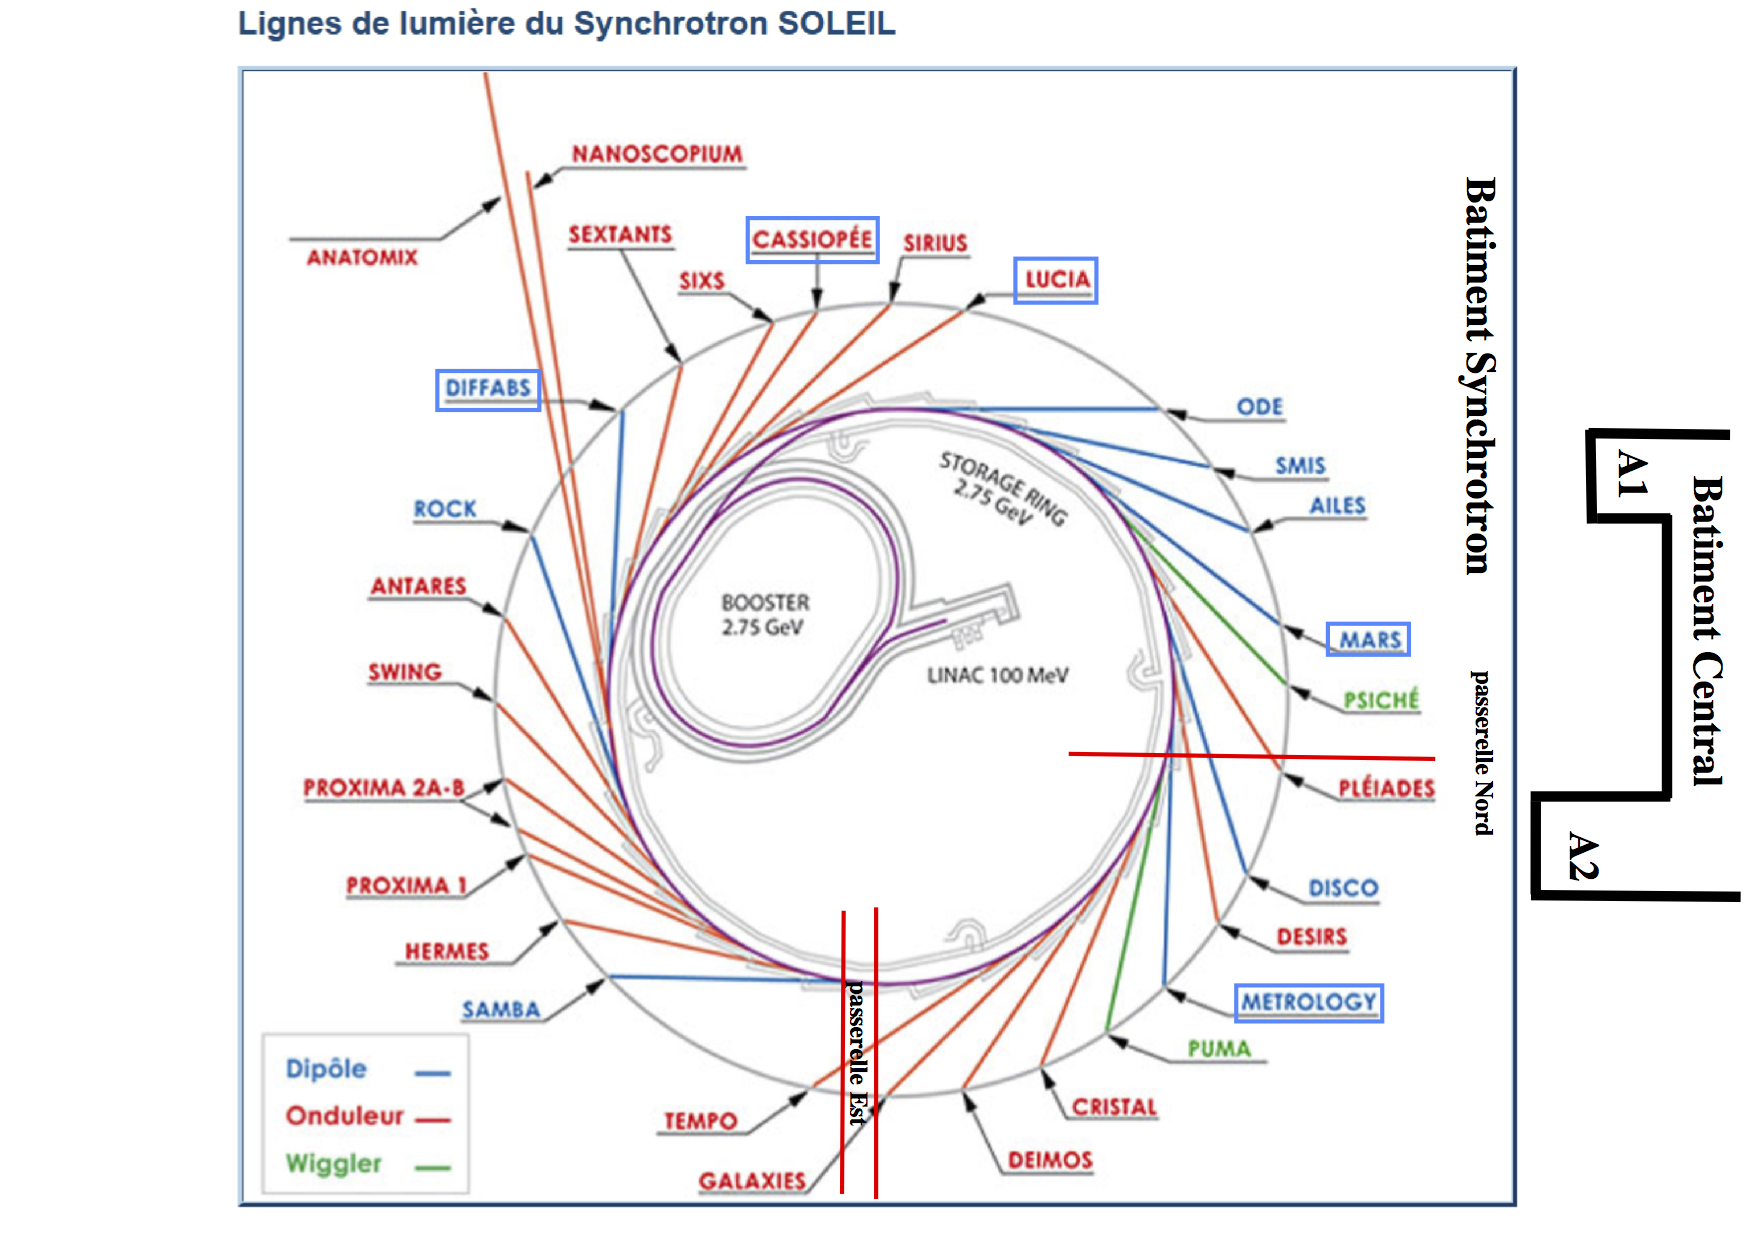
\includegraphics[width=16cm]{Chapitre2/planlignedelumieressoleil}}
  		 \caption{Lignes de lumière}
	\end{figure}


	
